\documentclass[12pt]{article}
\usepackage[spanish,es-nodecimaldot]{babel}
\usepackage[utf8]{inputenc}
\usepackage[T1]{fontenc}
\usepackage[a4paper,margin=2.5cm]{geometry}
\usepackage{lmodern}
\usepackage{setspace}
\usepackage{parskip}
\usepackage{graphicx}
\usepackage{float}
\usepackage{amsmath}
\usepackage{subcaption}
\setlength{\belowcaptionskip}{6pt}

\begin{document}
\renewcommand{\tablename}{Tabla}
\thispagestyle{empty}

\begin{center}
    \textsc{Universidad Central de Venezuela}\\[0.35cm]
    \textsc{Facultad de Ingenier\'ia}\\[0.35cm]
    \textsc{Escuela de Ingenier\'ia El\'ectrica}\\[0.35cm]
    \textsc{Departamento de Electr\'onica, Computaci\'on y Control}\\[0.35cm]
    \textsc{Laboratorio de Sistemas de Control I}
\end{center}

\vspace{5.5cm}

\begin{center}
    \textbf{QUANSER 2}
\end{center}

\vfill

\noindent
\begin{minipage}[t]{0.48\textwidth}
    \textbf{Aux. Docente:}\\[0.20cm]
    Gabriel Cumare
\end{minipage}%
\hfill
\begin{minipage}[t]{0.48\textwidth}
    \raggedleft
    \textbf{Alumna:}\\[0.20cm]
    Carla Fajardo V-27.571.576
\end{minipage}

\vspace{0.8cm}

\begin{center}
    Caracas, 2 de noviembre de 2026
\end{center}

\newpage
\tableofcontents
\newpage

\section{Introducci\'on}
En la ingenier\'ia de control, es fundamental lograr que los sistemas din\'amicos respondan de forma estable, precisa y eficiente. Cuando un sistema recibe una se\~nal de entrada, su salida no cambia instant\'aneamente: atraviesa un periodo transitorio, que puede incluir oscilaciones amortiguadas, antes de alcanzar el estado estacionario. La diferencia entre la salida alcanzada y la respuesta deseada en ese estado se conoce como error en estado estacionario y permite evaluar la precisi\'on del sistema. Por esta raz\'on, el dise\~no de un controlador debe considerar tanto la rapidez y estabilidad de la respuesta transitoria como la exactitud final.

Entre las estrategias de control m\'as utilizadas se encuentran las acciones proporcional (P), integral (I) y proporcional-integral (PI). La acci\'on proporcional responde al error presente y puede proporcionar una respuesta r\'apida, aunque por s\'i sola no siempre elimina el error en estado estacionario. La acci\'on integral acumula el error a lo largo del tiempo y puede reducirlo o eliminarlo, pero una sintonizaci\'on inadecuada puede ralentizar la respuesta o comprometer la estabilidad. El controlador PI combina ambas acciones para equilibrar rapidez y precisi\'on.

En este trabajo se analiza experimentalmente el comportamiento de las acciones P, I y PI aplicadas a un sistema din\'amico. Se comparan sus respuestas para identificar sus efectos sobre el comportamiento transitorio y el error en estado estacionario, y se relacionan las observaciones obtenidas con los principios fundamentales del control autom\'atico.

\newpage

\section{Objetivos}
El objetivo de la pr\'actica es que el estudiante analice sistemas de control mediante la simulaci\'on de los mismos utilizando el m\'odulo \textit{Quanser Engineering Trainer: DC Motor Control} como soporte. Se estudiar\'an los efectos en la respuesta transitoria de un sistema de control de velocidad de las acciones de control proporcional, integral y proporcional-integral.

\newpage

\section{Resultados}
\textbf{Trabajo de laboratorio}

\textbf{En cada caso imprima las gr\'aficas de las respuestas correspondientes.}

\subsection{Estudio de la acci\'on proporcional}

\noindent\textbf{3.1.1} Configure el m\'odulo DCMCT para control de velocidad en lazo cerrado, seleccionando la opci\'on \textit{Speed Control} en la esquina superior izquierda de la ventana del programa USB QICii. Active el funcionamiento del sistema con el icono \textit{Connect to Data Source}.

\noindent\textbf{3.1.2} Una vez activado el sistema, asigne los valores mostrados en la figura 1 para el generador de señales y el controlador en la ventana del USB QICii: 

\begin{figure}[H]
    \centering
    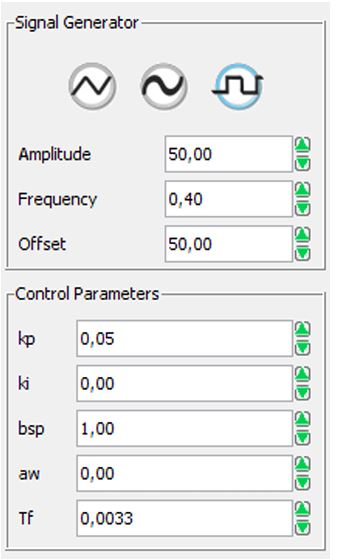
\includegraphics[width=0.3\textwidth]{imagenes/Controlador.JPG}
    \caption{Ventana del USB QICII.}
\end{figure}

\noindent\textbf{3.1.3} Var\'ie el valor de $K_p$ desde 0.05 hasta 0.40, con incrementos de 0.05, guardando las gr\'aficas correspondientes a la respuesta en cada caso. Si es necesario para visualizar el valor final de la respuesta, disminuya la frecuencia del generador de se\~nales.

\begin{figure}[H]
    \centering
    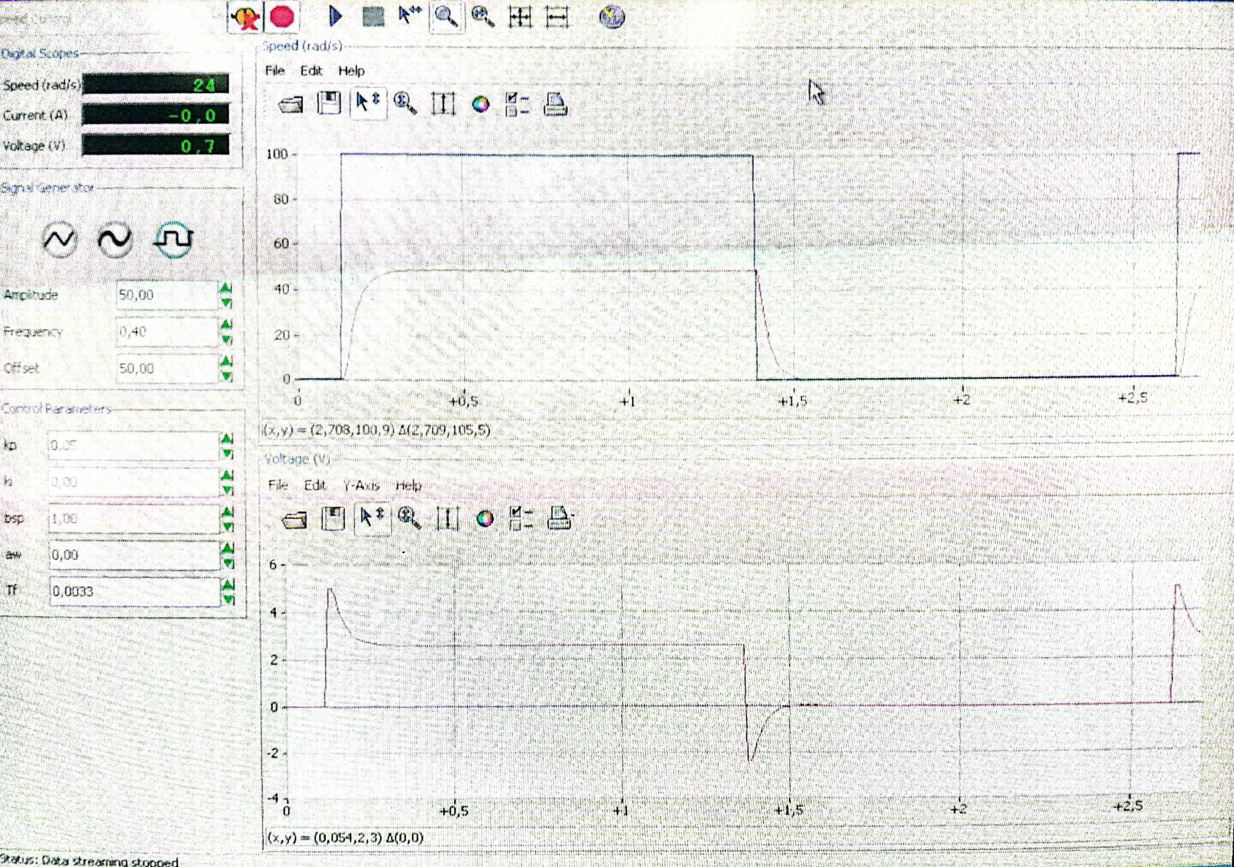
\includegraphics[width=0.5\textwidth]{imagenes/Kp_0.05.JPG}
    \caption{Respuesta del sistema para $K_p=0.05$.}
\end{figure}

\begin{figure}[H]
    \centering
    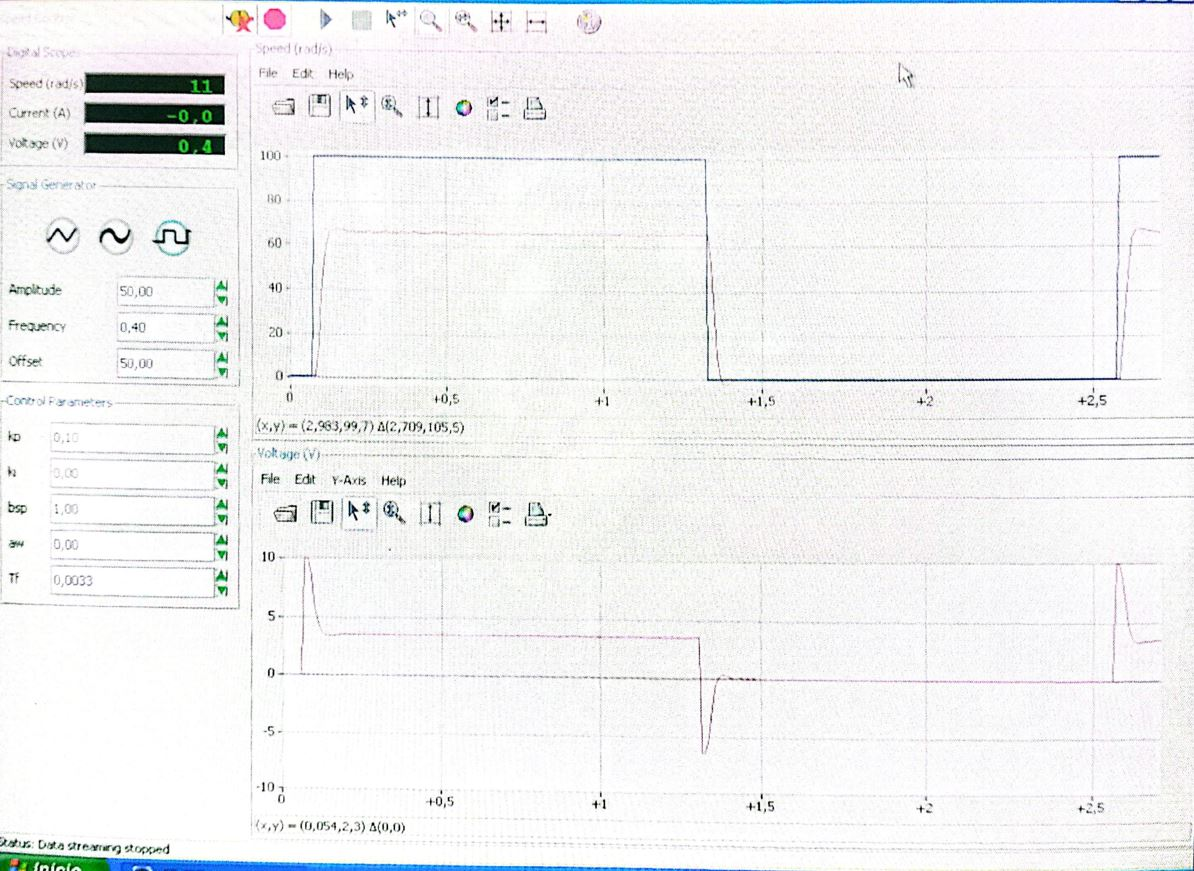
\includegraphics[width=0.5\textwidth]{imagenes/Kp_0.10.JPG}
    \caption{Respuesta del sistema para $K_p=0.10$.}
\end{figure}

\begin{figure}[H]
    \centering
    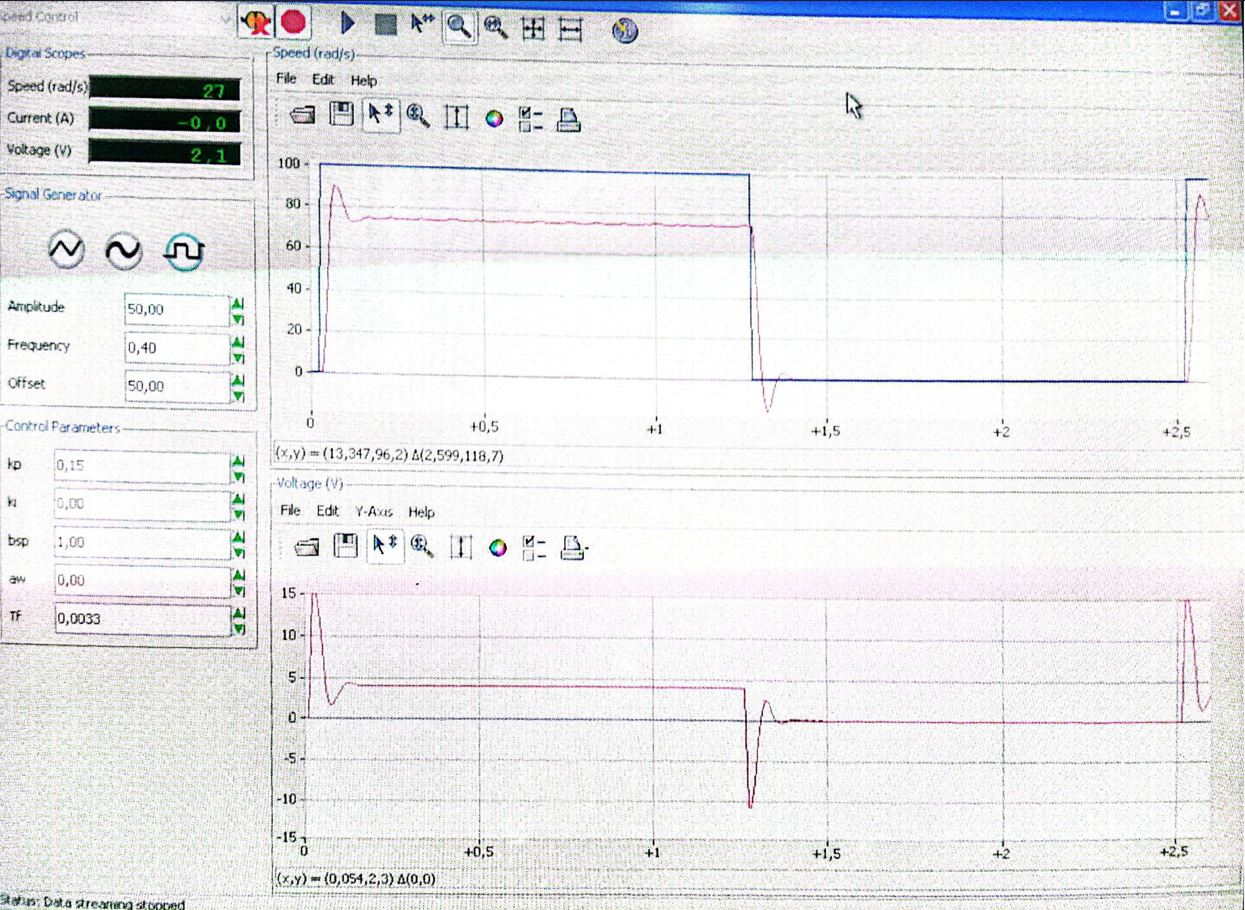
\includegraphics[width=0.5\textwidth]{imagenes/Kp_0.15.JPG}
    \caption{Respuesta del sistema para $K_p=0.15$.}
\end{figure}

\begin{figure}[H]
    \centering
    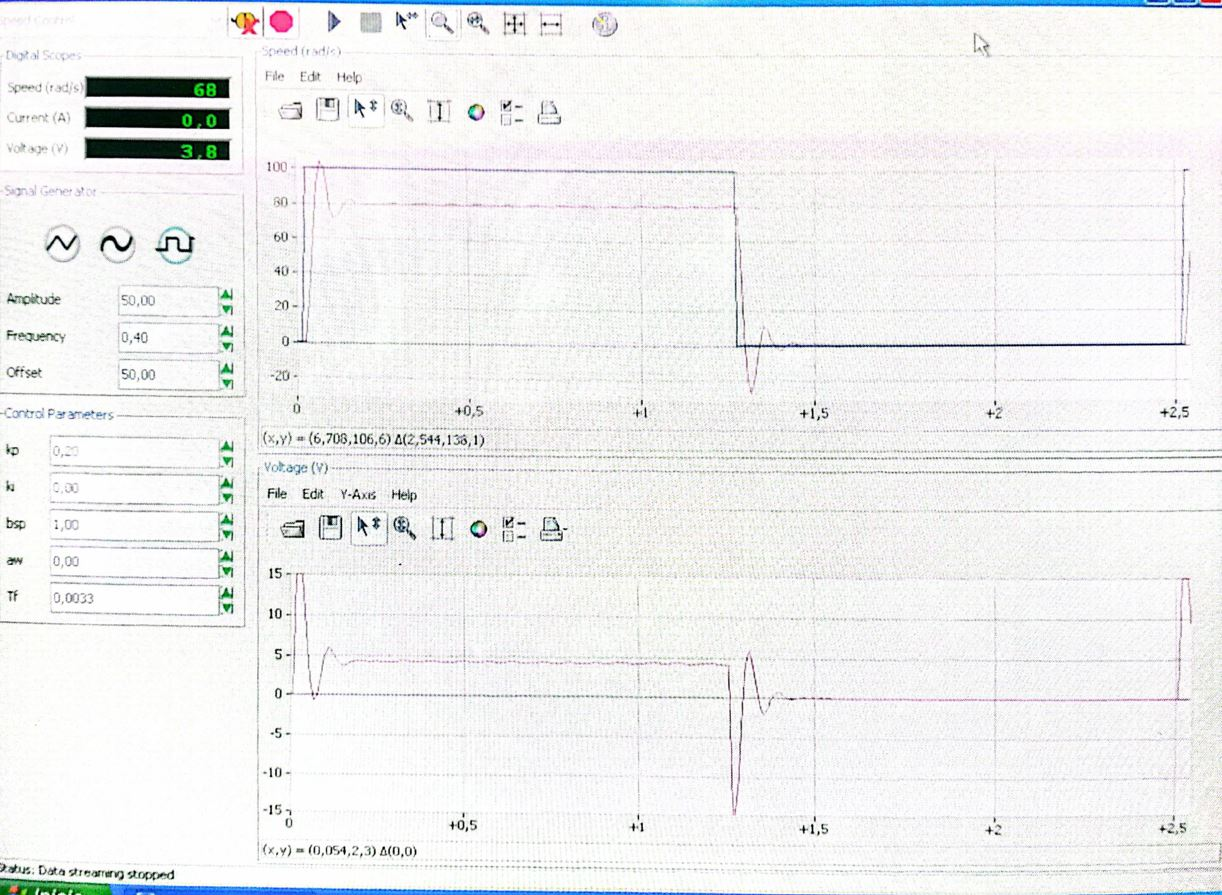
\includegraphics[width=0.5\textwidth]{imagenes/Kp_0.20.JPG}
    \caption{Respuesta del sistema para $K_p=0.20$.}
\end{figure}

\begin{figure}[H]
    \centering
    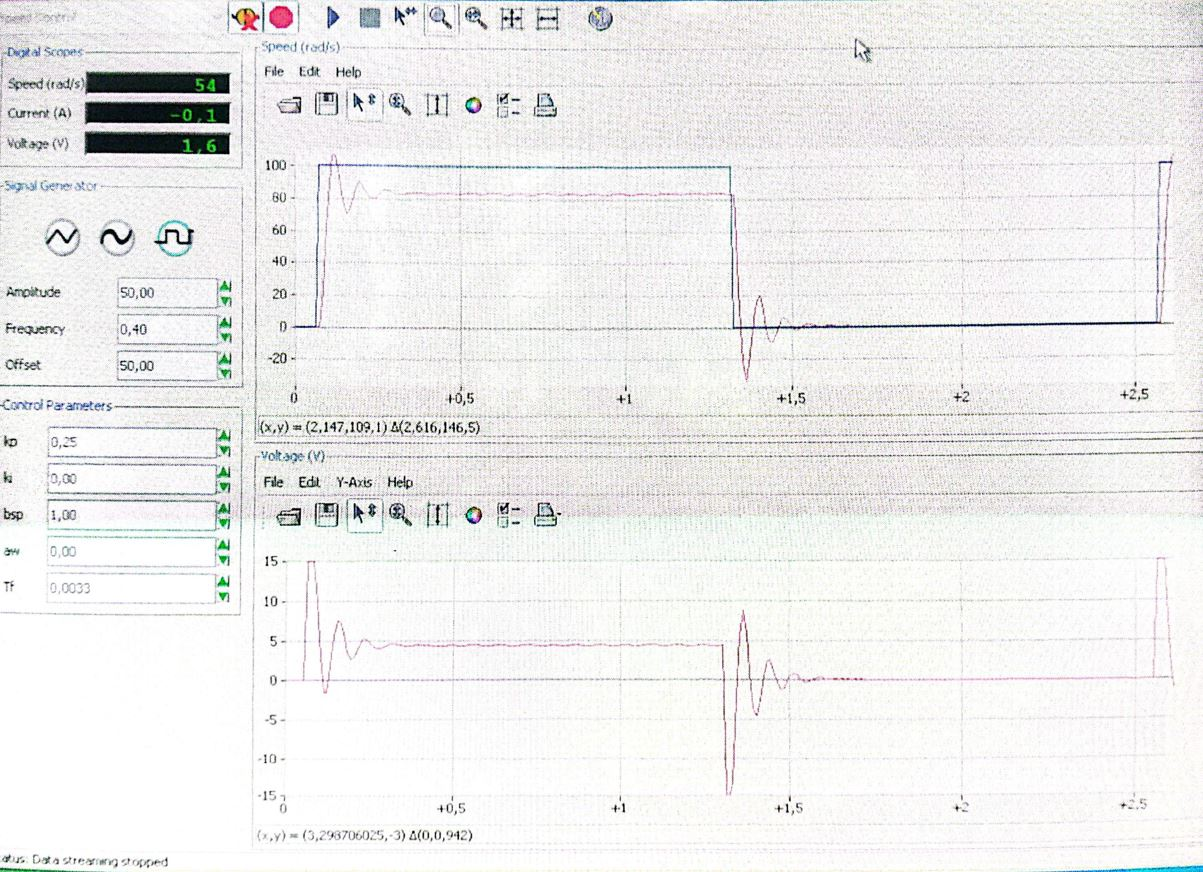
\includegraphics[width=0.5\textwidth]{imagenes/Kp_0.25.JPG}
    \caption{Respuesta del sistema para $K_p=0.25$.}
\end{figure}

\begin{figure}[H]
    \centering
    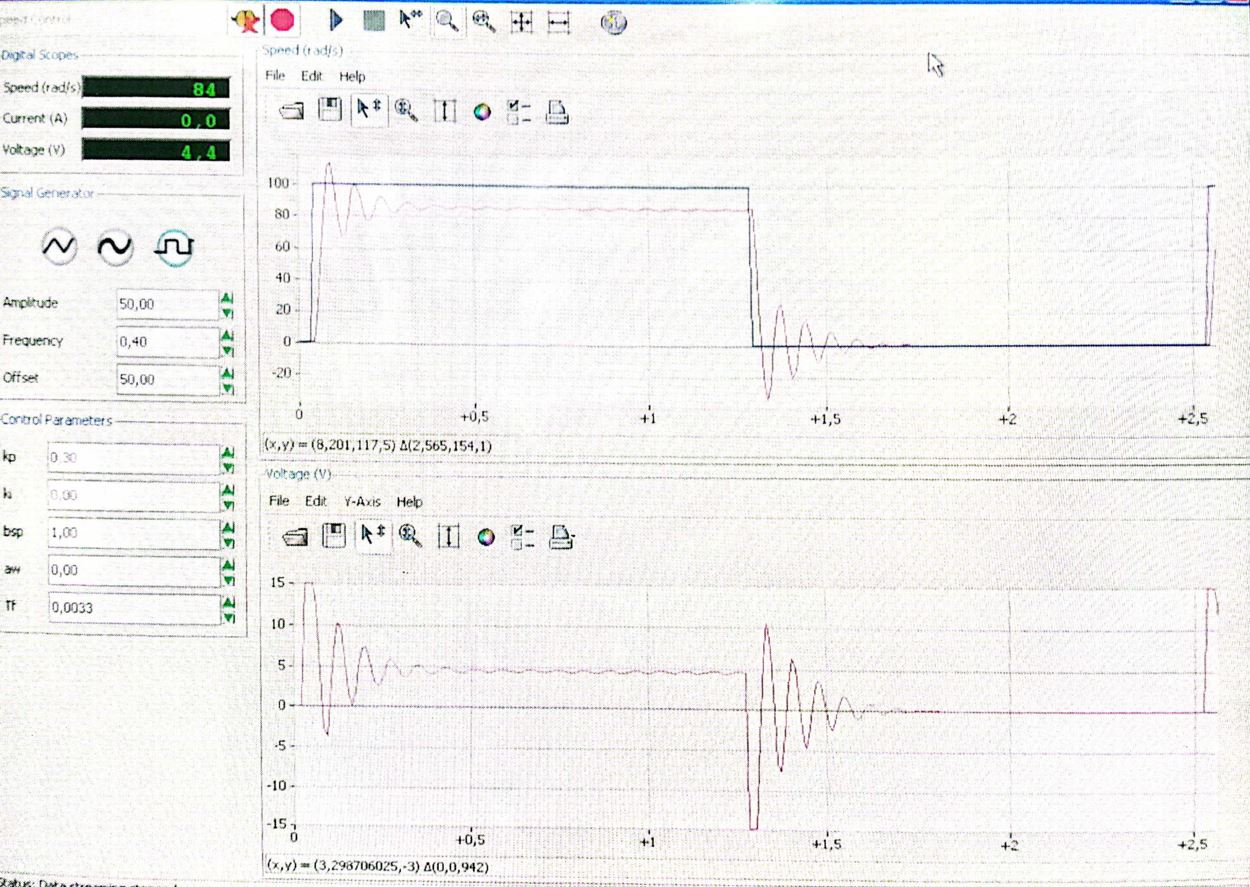
\includegraphics[width=0.5\textwidth]{imagenes/Kp_0.30.JPG}
    \caption{Respuesta del sistema para $K_p=0.30$.}
\end{figure}

\begin{figure}[H]
    \centering
    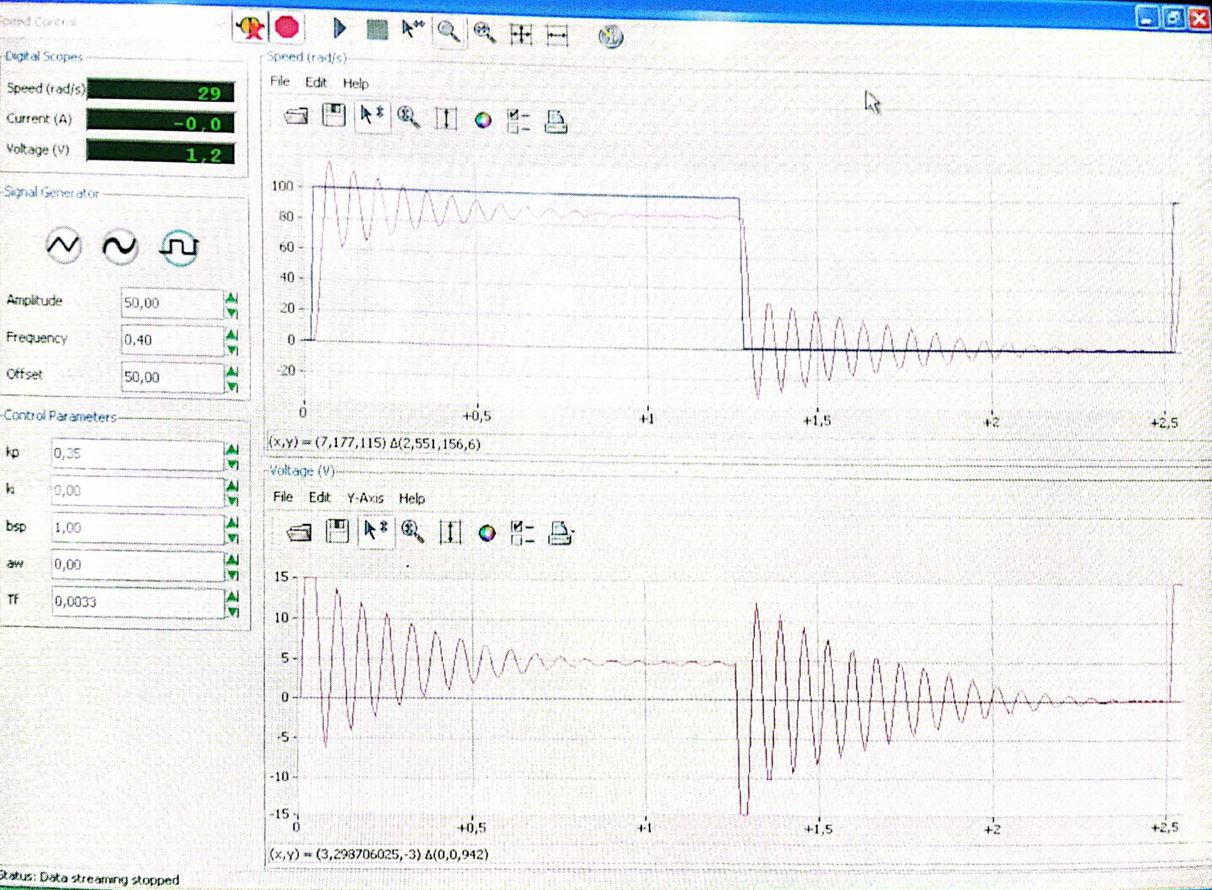
\includegraphics[width=0.5\textwidth]{imagenes/Kp_0.35.JPG}
    \caption{Respuesta del sistema para $K_p=0.35$.}
\end{figure}

\begin{figure}[H]
    \centering
    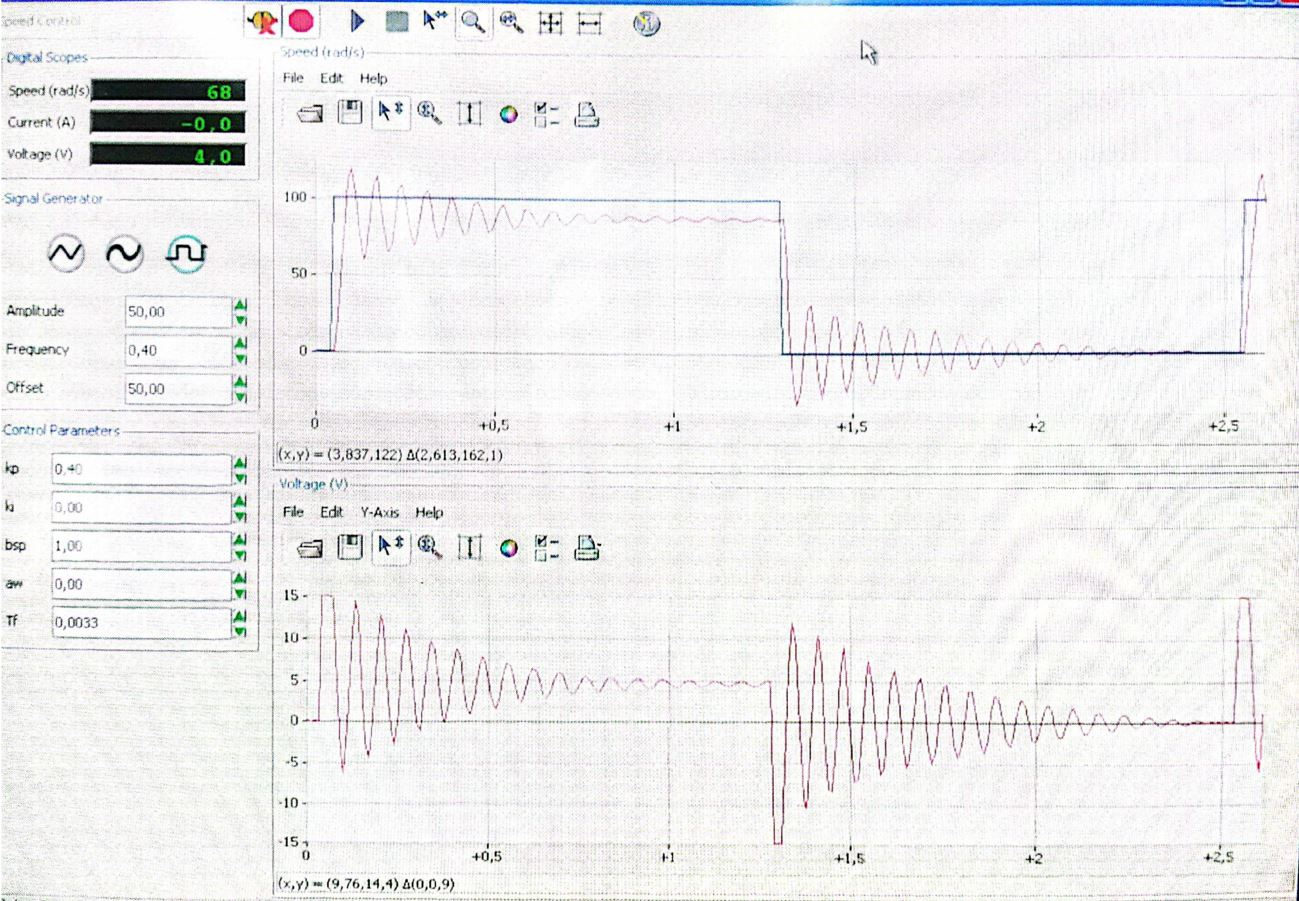
\includegraphics[width=0.5\textwidth]{imagenes/Kp_0.40.JPG}
    \caption{Respuesta del sistema para $K_p=0.40$.}
\end{figure}

\noindent Al aumentar el valor de $K_p$, la respuesta transitoria del sistema se vuelve m\'as lenta, con menor tiempo de subida pero mayor tiempo de estabilizaci\'on; sin embargo, tambi\'en aumenta el sobreimpulso y las oscilaciones, lo que indica un comportamiento m\'as cercano a un sistema inestable. Adem\'as, el error en estado estacionario disminuye, lo cual es caracter\'istico de un controlador proporcional. 
\subsection{Estudio de la acci\'on integral}

\noindent\textbf{3.2.1} Con el sistema activo y la configuraci\'on para el generador de se\~nales anterior, configure el controlador asignando cero en los par\'ametros $K_p$, $b_{sp}$ y $a_w$. Para la ganancia del integrador asigne $K_i=0.1$.

\medskip

\noindent\textbf{3.2.2} Var\'ie $K_i$ desde 0.1 hasta 2.8 con incrementos de 0.3. Presente los resultados obtenidos en cada caso de acuerdo con las instrucciones indicadas en el punto 3.1.3. Disminuya la frecuencia del generador de se\~nales de ser necesario para la visualizaci\'on del valor final.

\begin{figure}[H]
    \centering
    \includegraphics[width=0.5\textwidth]{\detokenize{imagenes/Quanser II - Informe/Ki_0.10.JPG}}
    \caption{Respuesta del sistema para $K_i=0.1$.}
\end{figure}

\begin{figure}[H]
    \centering
    \includegraphics[width=0.5\textwidth]{\detokenize{imagenes/Quanser II - Informe/Ki_0.40.JPG}}
    \caption{Respuesta del sistema para $K_i=0.4$.}
\end{figure}

\begin{figure}[H]
    \centering
    \includegraphics[width=0.5\textwidth]{\detokenize{imagenes/Quanser II - Informe/Ki_0.7.JPG}}
    \caption{Respuesta del sistema para $K_i=0.7$.}
\end{figure}

\begin{figure}[H]
    \centering
    \includegraphics[width=0.5\textwidth]{\detokenize{imagenes/Quanser II - Informe/Ki_1.0.JPG}}
    \caption{Respuesta del sistema para $K_i=1.0$.}
\end{figure}

\begin{figure}[H]
    \centering
    \includegraphics[width=0.5\textwidth]{\detokenize{imagenes/Quanser II - Informe/Ki_1.3.JPG}}
    \caption{Respuesta del sistema para $K_i=1.3$.}
\end{figure}

\begin{figure}[H]
    \centering
    \includegraphics[width=0.5\textwidth]{\detokenize{imagenes/Quanser II - Informe/Ki_1.6.JPG}}
    \caption{Respuesta del sistema para $K_i=1.6$.}
\end{figure}

\begin{figure}[H]
    \centering
    \includegraphics[width=0.5\textwidth]{\detokenize{imagenes/Quanser II - Informe/Ki_1.9.JPG}}
    \caption{Respuesta del sistema para $K_i=1.9$.}
\end{figure}

\begin{figure}[H]
    \centering
    \includegraphics[width=0.5\textwidth]{\detokenize{imagenes/Quanser II - Informe/Ki_2.2.JPG}}
    \caption{Respuesta del sistema para $K_i=2.2$.}
\end{figure}

\begin{figure}[H]
    \centering
    \includegraphics[width=0.5\textwidth]{\detokenize{imagenes/Quanser II - Informe/Ki_2.5.JPG}}
    \caption{Respuesta del sistema para $K_i=2.5$.}
\end{figure}

\begin{figure}[H]
    \centering
    \includegraphics[width=0.5\textwidth]{\detokenize{imagenes/Quanser II - Informe/Ki_2.8.JPG}}
    \caption{Respuesta del sistema para $K_i=2.8$.}
\end{figure}

\noindent Como se puede observar en las graficas anteriores, la ganancia integral elevada puede aumentar el sobreimpulso y las
oscilaciones así como también prolongar el tiempo de estabilización. Por otro lado, al aumentar $K_i$, la acción integral corrige completamente el error en estado estacionario ya que el el sistema pasa a ser de tipo 0 a tipo 1.

\subsection{Estudio de la acci\'on proporcional integral}

\noindent\textbf{3.3.1} Mantenga en cero los par\'ametros $b_{sp}$ y $a_w$. Calcule los valores de $K_p$ y $K_i$ necesarios para mantener la misma din\'amica observada en el caso de $K_p=0.24$ utilizando control proporcional.

\begin{figure}[H]
	    \centering
        \includegraphics[width=0.5\textwidth]{\detokenize{imagenes/Quanser II - Informe/3Kp_0.24.JPG}}
        \caption{$K_p=0.24$.}
\end{figure}

\begin{figure}[H]
	\centering
    \begin{subfigure}[b]{0.4\textwidth}
        \centering
        \includegraphics[width=\textwidth]{\detokenize{imagenes/Quanser II - Informe/Kp_0.10_Ki_2.60.JPG}}
        \caption{$K_p=0.18,\ K_i=2.60$.}
    \end{subfigure}
    \hfill
    \begin{subfigure}[b]{0.4\textwidth}
        \centering
        \includegraphics[width=\textwidth]{\detokenize{imagenes/Quanser II - Informe/mKi_3.60_Kp_0.08.JPG}}
        \caption{$K_p=0.08, \ K_i=3.60$.}
    \end{subfigure}
    \caption{Comparaci\'on de respuestas en el apartado 3.3.1.}
\end{figure}

\begin{table}[H]
    \centering
    \caption{Par\'ametros y caracter\'isticas de las respuestas en el apartado 3.3.1.}
    \small
    \begin{tabular}{c|cc|cccc}
        \hline
        Caso & $K_p$ & $K_i$ & $t_p$ (s) & $t_s$ (s) & $M$ (\%) & $t_r$ (s) \\
        \hline
        Proporcional & 0,24 & 0 & 1,88 & 2,054 & 38,80 & 1,859 \\
        PI 1 & 0,18 & 2,60 & 3,358 & 4,52 & 50,80 & 3,06 \\
        PI 2 & 0,08 & 3,60 & 2,75 & 3,22 & 25,251 & 2,31 \\
        \hline
    \end{tabular}
\end{table}

\noindent Al comparar la figura 20, correspondiente al control proporcional con $K_p=0.24$, con la figura 21(b), correspondiente al control PI con $K_p=0.08$ y $K_i=3.60$, se observa un compromiso entre rapidez y amortiguamiento. Según los valores de la tabla 1, el control proporcional presenta un tiempo de subida menor ($1.859$ s frente a $2.31$ s) y se estabiliza antes ($2.054$ s frente a $3.22$ s). En cambio, la respuesta PI tiene un sobreimpulso menor ($25.251\%$ frente a $38.80\%$), aunque tarda más en alcanzar y estabilizarse alrededor de la referencia. Además, en las gráficas el control PI mantiene la salida más cerca del valor de referencia en estado estacionario, mientras que con control proporcional se aprecia un error residual. Por tanto, en estas condiciones el PI ofrece menor sobreimpulso y mejor precisión final, a costa de una respuesta transitoria más lenta.

\medskip

\noindent\textbf{3.3.2} Ajuste en el controlador los valores m\'as cercanos posibles a los obtenidos en 3.3.1. Observe el resultado obtenido en el sistema y compare con el caso indicado de la acci\'on proporcional. En el generador de se\~nales asigne 0 a la amplitud y el offset; una vez detenido el motor, asigne 50 al offset y registre el resultado observado.

\begin{figure}[H]
    \centering
    \includegraphics[width=0.6\textwidth]{\detokenize{imagenes/Quanser II - Informe/offset_50.JPG}}
    \caption{Respuesta del sistema con offset de 50.}
\end{figure}

\begin{table}[H]
    \centering
    \caption{Frecuencia natural para cada tipo de control.}
    \begin{tabular}{c|c}
        \hline
        Control & $\omega_n$ (rad/s) \\
        \hline
        PI & 130 \\
        I & 120 \\
        \hline
    \end{tabular}
\end{table}

\newpage

\section{An\'alisis de Resultados}
\subsection{Acci\'on proporcional}
Al variar $K_p$ entre 0.05 y 0.40 se observa que la ganancia proporcional modifica tanto la rapidez como el amortiguamiento de la respuesta. En general, al aumentar $K_p$ el controlador act\'ua directamente ante el error, lo que tiende a reducir el tiempo de subida y el error en estado estacionario. Sin embargo, una ganancia elevada puede producir mayor sobreimpulso y oscilaciones, y prolongar el tiempo necesario para que la respuesta se estabilice. Este compromiso entre rapidez y amortiguamiento se aprecia en las respuestas registradas. El error no desaparece necesariamente con control proporcional, por lo que queda un error residual en r\'egimen permanente.

\subsection{Acci\'on integral}
En el control integral, aumentar $K_i$ fortalece la correcci\'on del error acumulado, eliminando el error en estado estacionario ante una referencia constante, siempre que el sistema permanezca estable. A cambio, valores altos de $K_i$ pueden incrementar el sobreimpulso y las oscilaciones, adem\'as de alargar el tiempo de estabilizaci\'on. Las respuestas experimentales muestran la importancia de ajustar esta ganancia: una correcci\'on integral m\'as intensa no implica necesariamente una respuesta transitoria mejor amortiguada.

\subsection{Acci\'on proporcional-integral}
El controlador PI combina la respuesta inmediata de la acci\'on proporcional con la capacidad de la integral para corregir el error acumulado. La comparaci\'on cuantitativa de la secci\'on 3.3 muestra que el caso proporcional ($K_p=0.24$, $K_i=0$) tiene $t_r=1.859$ s, $t_s=2.054$ s y un sobreimpulso de $38.80\%$. Para $K_p=0.18$ y $K_i=2.60$, estos valores son $3.06$ s, $4.52$ s y $50.80\%$, respectivamente: esta sintonizaci\'on presenta una respuesta m\'as lenta y un sobreimpulso mayor que el caso proporcional. En cambio, con $K_p=0.08$ y $K_i=3.60$, el tiempo de subida es $2.31$ s, el tiempo de estabilizaci\'on es $3.22$ s y el sobreimpulso es $25.251\%$. En este \'ultimo caso se reduce el sobreimpulso, aunque la respuesta sigue siendo m\'as lenta que la proporcional de referencia. Los resultados evidencian que el comportamiento del PI depende de la combinaci\'on de ambas ganancias y que su ajuste requiere equilibrar rapidez, sobreimpulso y estabilizaci\'on.

Por \'ultimo, la tabla de la secci\'on 3.3 registra frecuencias naturales de $130$ rad/s para PI y $120$ rad/s para control integral. La diferencia es de $10$ rad/s, con un valor ligeramente mayor para PI. En conjunto, las mediciones confirman que incorporar la acci\'on proporcional cambia la din\'amica transitoria, mientras que la acci\'on integral aporta correcci\'on del error en r\'egimen permanente; la sintonizaci\'on debe seleccionarse seg\'un el compromiso requerido entre precisi\'on y rapidez.

\newpage

\section{Conclusiones}
Los resultados de la pr\'actica permitieron cumplir el objetivo de analizar experimentalmente el efecto de las acciones proporcional, integral y proporcional-integral sobre la respuesta de velocidad del motor, tanto en el periodo transitorio como en el estado estacionario. El control proporcional ofrece una respuesta inicial directa y puede mejorar su rapidez al ajustar $K_p$; sin embargo, por s\'i solo no elimina necesariamente el error permanente, y valores de ganancia elevados pueden producir mayor sobreimpulso y oscilaciones.

La acci\'on integral act\'ua sobre el error acumulado y permite reducir el error en estado estacionario, aunque al aumentar $K_i$ puede hacer m\'as oscilatoria la respuesta y prolongar su estabilizaci\'on. Por ello, ni la acci\'on proporcional ni la integral, consideradas de manera aislada, garantizan por s\'i mismas el mejor desempe\~no en todos los aspectos. El controlador PI combina ambas acciones: la proporcional responde al error presente y la integral corrige el error acumulado. No obstante, las mediciones muestran que el resultado depende de la sintonizaci\'on y que la combinaci\'on no es necesariamente m\'as r\'apida que el control proporcional.

En particular, el ajuste PI con $K_p=0.18$ y $K_i=2.60$ present\'o un sobreimpulso de $50.80\%$ y un tiempo de estabilizaci\'on de $4.52$ s. Con $K_p=0.08$ y $K_i=3.60$, el sobreimpulso baj\'o a $25.251\%$ y el tiempo de estabilizaci\'on fue de $3.22$ s; aun as\'i, este \'ultimo tiempo fue mayor que los $2.054$ s registrados con control proporcional para $K_p=0.24$. La comparaci\'on evidencia el compromiso entre rapidez, sobreimpulso y precisi\'on, y la necesidad de seleccionar $K_p$ y $K_i$ de acuerdo con el comportamiento deseado. En conjunto, la experiencia permiti\'o observar estos compromisos y relacionar las respuestas medidas con el funcionamiento de cada tipo de controlador.

\newpage

\section{Anexos}
\begin{center}
    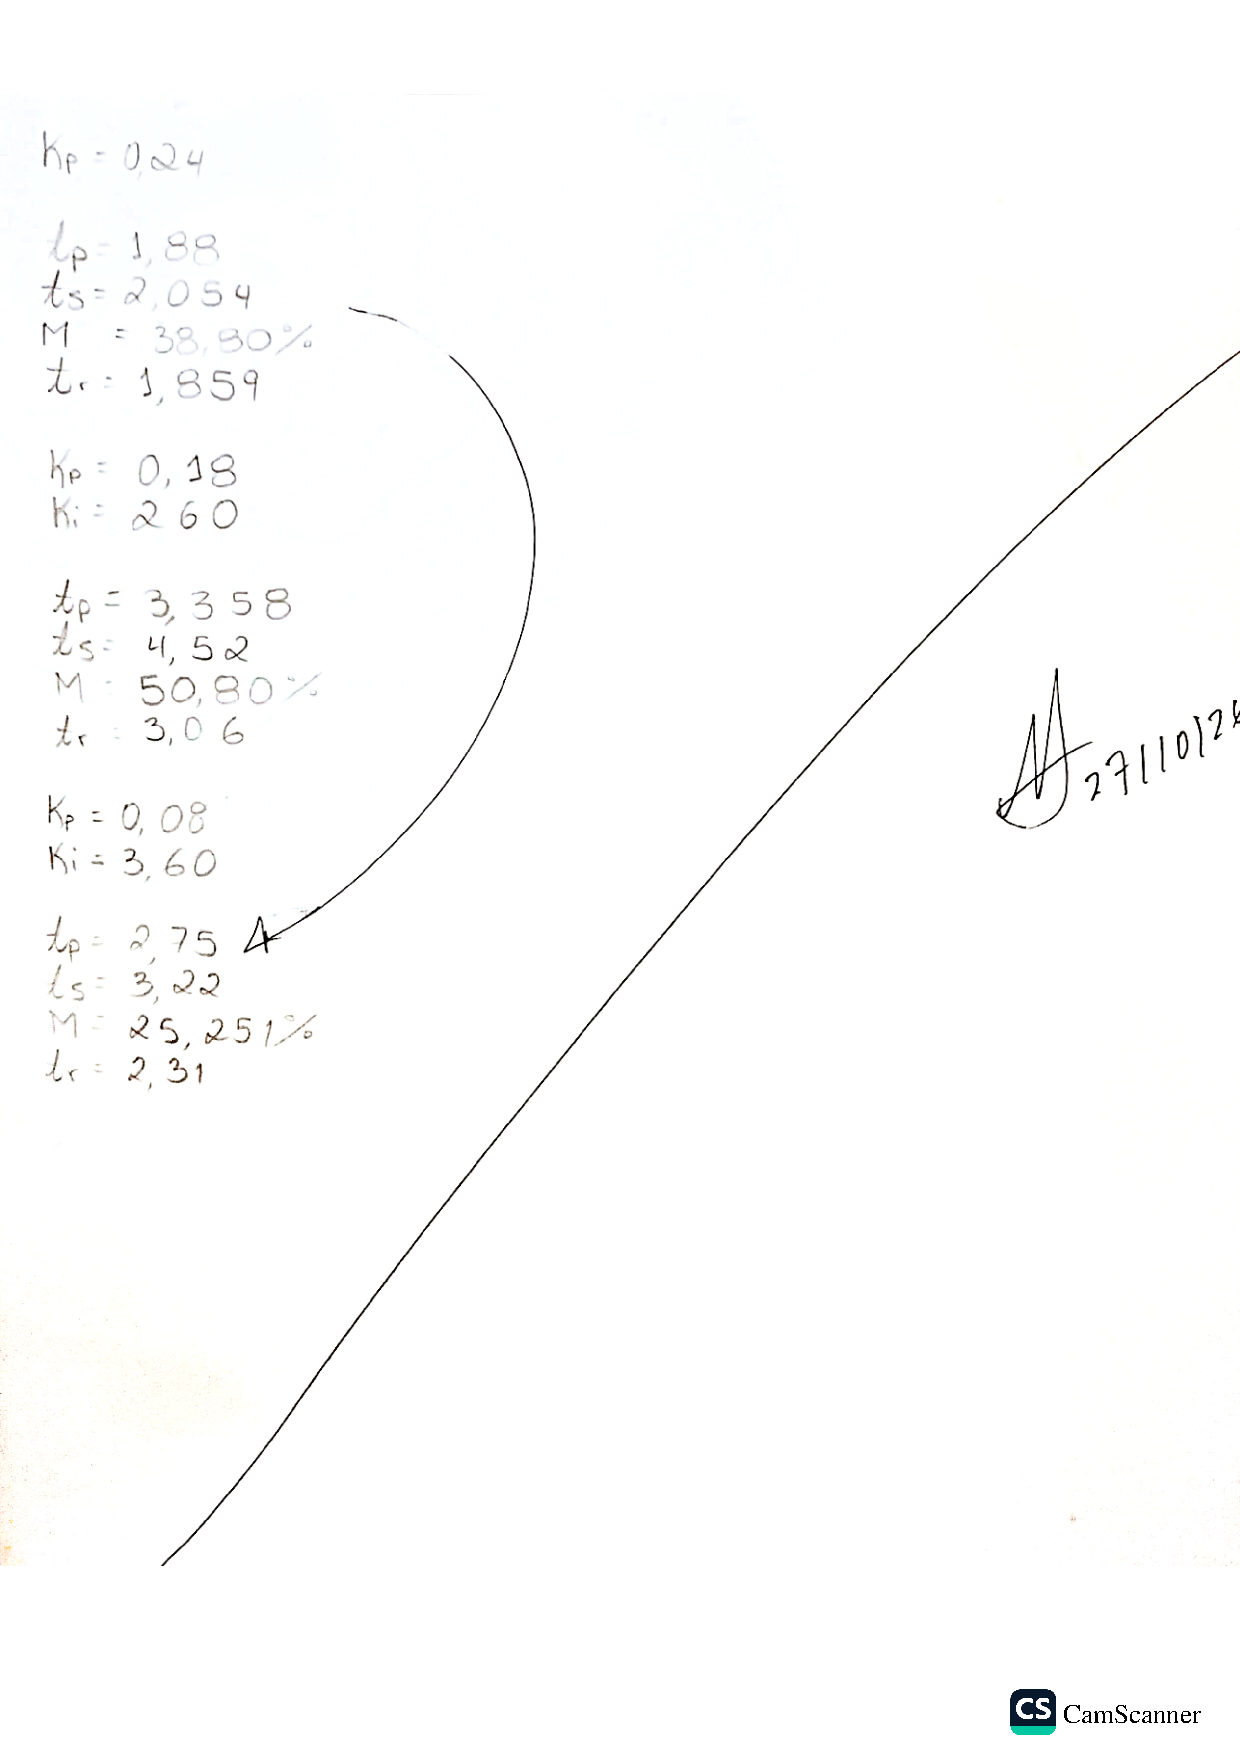
\includegraphics[page=1,width=\textwidth,height=0.78\textheight,keepaspectratio]{Anexo_CamScanner.pdf}
\end{center}

\end{document}
